\documentclass[xcolor=table,t,aspectratio=169]{beamer}
\usepackage{pgfpages,graphicx,listings,hyperref}
\usepackage{subfigure}
\usepackage[table]{xcolor}
\usepackage{multicol,multirow}
\usepackage{listings}
\usepackage{tikz}
\usetikzlibrary{positioning}
\usepackage{tcolorbox}
\usepackage{enumerate}
\definecolor{gray}{rgb}{0.4,0.4,0.4}
\definecolor{darkblue}{rgb}{0.0,0.0,0.6}
\definecolor{cyan}{rgb}{0.0,0.6,0.6}
\definecolor{ugmyellow}{HTML}{f6d648}
\definecolor{ugmblue}{HTML}{194168}
\definecolor{ugmbackgroundblue}{HTML}{00416B}
\definecolor{ugmbackgroundgrey}{RGB}{220, 220, 220}
\renewcommand{\figurename}{Gambar}

\lstdefinelanguage{C++}
{
	stringstyle=\color{black},
	identifierstyle=\color{darkblue},
	keywordstyle=\color{cyan},
	morekeywords={cin,cout}% list your attributes here
}

\lstset{language=SQL,
	columns=fullflexible,
	showstringspaces=false,
	numbers=left,   
	numbersep=5pt,frame=single,stepnumber=3,
	basicstyle=\ttfamily,
	keywordstyle=\color{blue}\ttfamily,
	stringstyle=\color{red}\ttfamily,
	commentstyle=\color{cyan}\ttfamily,
	morecomment=[l][\color{magenta}]{\#}
}

\usepackage[utf8]{inputenc}
\hypersetup{%
	pdftitle={Data Warehouse \& Business Intelligence},%
	pdfauthor={Khabib Mustofa,Dr.techn.},%
	pdfsubject={Kuliah S2 Ilmu Komputer},%
	pdfkeywords={Warehouse, OLAP, Data Mart}%
}
\definecolor{links}{HTML}{2A1B81}
\hypersetup{colorlinks,linkcolor=,urlcolor=links}
\setbeamercovered{transparent}

\definecolor{ag}{rgb}{0.55, 0.71, 0.0}
\newcommand{\teksmerah}[1]{{\color{red} #1}}
\newcommand{\teksbiru}[1]{{\color{blue} #1}}
\newcommand{\tekshijau}[1]{{\color{ag} #1}}
\newcommand{\kodependek}[1]{{\teksbiru{\texttt{#1}}}}
\newcommand{\kodemerah}[1]{{\teksmerah{\texttt{#1}}}}
  \newcommand{\tebalmerah}[1]{{\bfseries\color{red} #1}}
\newcommand{\tebalbiru}[1]{{\bfseries\color{blue} #1}}
\newcommand{\tebalhijau}[1]{{\bfseries\color{ag} #1}}

%$$$$$$$$$$$$$$$$
\title[Data Mart Bus Antarkota]{Data Mart dan Visualisasi Perjalanan Bus Antarkota}
\subtitle{Perjalanan Multi-Leg dan Loyalitas Penumpang}
\date{}
\author[Citra dan Ade]{Citra Putri Saragih \\ Ade Dwi Putra}
\institute[UGM]{Data Warehouse \& Business Intelligence\\Universitas Gadjah Mada}
% Beginning of Code for UGM 2025 Template
\usefonttheme{professionalfonts}
\setbeamerfont{title}{series=\bfseries,parent=structure}
\setbeamerfont{frametitle}{series=\bfseries,parent=structure}
\mode<article> % only for the article version
{
  \usepackage{fullpage}
  \usepackage{hyperref}
}

\mode<presentation>
{
 \logo{
\includegraphics[height=.75cm]{images/logougm.png}}
}
\usetheme{Copenhagen}
\usecolortheme{seahorse}
\definecolor{ugmyellow}{HTML}{f6d648}
\definecolor{ugmblue}{HTML}{194168}
\definecolor{ugmbackgroundblue}{HTML}{00416B}
\definecolor{ugmgray}{HTML}{E0E0E0}
\setbeamercolor{title}{bg=ugmgray, fg=ugmblue}
\setbeamercolor{frametitle}{bg=white, fg=ugmblue}
\setbeamercolor{section in head/foot}{fg=white, bg=ugmblue}
\setbeamercolor{subsection in head/foot}{fg=black, bg=ugmgray}
\setbeamertemplate{blocks}[rounded][shadow=true]

% Regular block
\setbeamercolor{block title}{fg=white, bg=ugmblue}
\setbeamercolor{block body}{fg=black, bg=ugmblue!8}
\setbeamertemplate{footline}{
  \leavevmode%
  \hbox{%
    % Column 1: 60% - White on darkblue
    \colorbox{ugmgray}{\makebox[.50\paperwidth][l]{   \color{ugmblue}\hspace{2ex}\usebeamerfont{author in head/foot}%
      \textbf{Merakyat, Mandiri, Berkelanjutan $|$ Inclusive, Self-Reliant, Sustainable}
    }}%
    
    % Column 2: 25% - Black on grey
    \colorbox{ugmbackgroundblue}{\makebox[.15\paperwidth][c]{
      \color{white}\usebeamerfont{title in head/foot}%
      \textbf{ugm.ac.id}
    }}%
    
    % Column 3: 15% - White on darkblue
    \colorbox{ugmgray}{\makebox[.40\paperwidth][c]{
  \color{black}\usebeamerfont{date in head/foot}%
  \textbf{\insertshorttitle\ (\insertframenumber/\inserttotalframenumber) \hspace{2ex}}%
}}
  }%
  \vskip0pt%
}
\usebackgroundtemplate{\tikz\node[opacity=0.2]{
\includegraphics[height=\paperheight]{images/latar31.jpg}};}
% End of Code for UGM 2025 Template
%$$$$$$$$$$$$$$$$$$
\setbeamertemplate{caption}[numbered]
\AtBeginSection[]
{
   \begin{frame}
       \frametitle{Cakupan Materi}
       \tiny
       \tableofcontents[currentsection]
   \end{frame}
}


\begin{document}
\frame{ \titlepage}

\section{Kebutuhan Bisnis}

\begin{frame}{Domain dan Ruang Lingkup}
\footnotesize
Domain yang dipilih adalah perjalanan bus antarkota yang dapat terdiri atas
beberapa segmen (\textit{multi-leg}) dan melibatkan transit antarterminal.

\vspace{0.4cm}
Ruang lingkupnya meliputi:
\begin{enumerate}
    \item penjualan tiket;
    \item pelaksanaan perjalanan per segmen; dan
    \item transaksi loyalitas penumpang.
\end{enumerate}

Seluruh data dalam studi kasus dibuat secara sintetis.
\end{frame}

\begin{frame}{Masalah Bisnis}
\footnotesize
\begin{columns}[T]
\column{0.32\textwidth}
\begin{block}{Operasional}
Keterlambatan, waktu transit, dan \textit{missed connection}.
\end{block}
\column{0.32\textwidth}
\begin{block}{Komersial}
Pendapatan serta kerugian akibat \textit{refund}, pemesanan ulang, dan kompensasi.
\end{block}
\column{0.32\textwidth}
\begin{block}{Loyalitas}
Aktivitas poin dan hubungan gangguan perjalanan dengan pemesanan kembali.
\end{block}
\end{columns}

\vspace{0.5cm}
Data mart diperlukan untuk menggabungkan ketiga sudut pandang tersebut dalam
analisis historis.
\end{frame}

\begin{frame}{Stakeholder dan Business Questions}
\footnotesize
\begin{tabular}{|p{3.7cm}|p{10cm}|}
\hline
\textbf{Stakeholder} & \textbf{Kebutuhan utama} \\ \hline
VP of Operations & Terminal dan pasangan rute dengan \textit{missed connection};
rute dan armada dengan keterlambatan serta pelanggaran SLA. \\ \hline
VP Commercial \& Revenue & Nilai \textit{revenue leakage} pada musim sibuk. \\ \hline
Head of Customer Loyalty & Perbedaan perilaku per tingkat loyalitas dan asosiasi
gangguan perjalanan dengan \textit{repeat booking}. \\ \hline
\end{tabular}

\vspace{0.4cm}
Lima pertanyaan bisnis tersebut menjadi dasar desain dan query verifikasi.
\end{frame}

\section{Perancangan Dimensional}

\begin{frame}{Grain Setiap Fact Table}
\footnotesize
\begin{tabular}{|p{5cm}|p{8.7cm}|}
\hline
\textbf{Fact table} & \textbf{Grain} \\ \hline
\texttt{fct\_ticket\_sales} & Satu tiket milik satu penumpang pada satu segmen
saat pembelian. \\ \hline
\texttt{fct\_passenger\_itinerary\_leg} & Satu penumpang pada satu segmen dalam
satu perjalanan terjadwal. \\ \hline
\texttt{fct\_loyalty\_transaction} & Satu mutasi poin milik satu penumpang. \\ \hline
\end{tabular}

\vspace{0.4cm}
Grain atomik dipilih agar data dapat diringkas berdasarkan tanggal, terminal,
rute, armada, maupun penumpang.
\end{frame}

\begin{frame}{Dimensional Model}
\centering
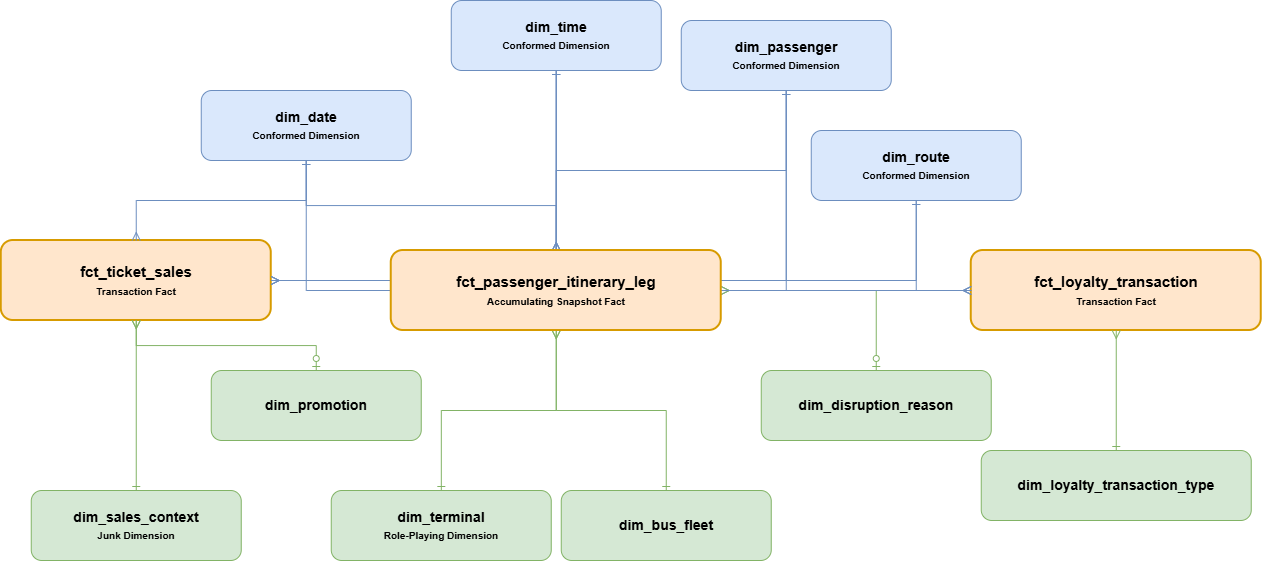
\includegraphics[width=0.9\textwidth,height=0.65\textheight,keepaspectratio]
{figures/dimensional_model.png}
\vspace{0.2cm}

\footnotesize Diagram konseptual memperlihatkan tiga fact table dan conformed
dimensions yang digunakan bersama.
\end{frame}

\begin{frame}{Dimensional Model Lengkap}
\centering
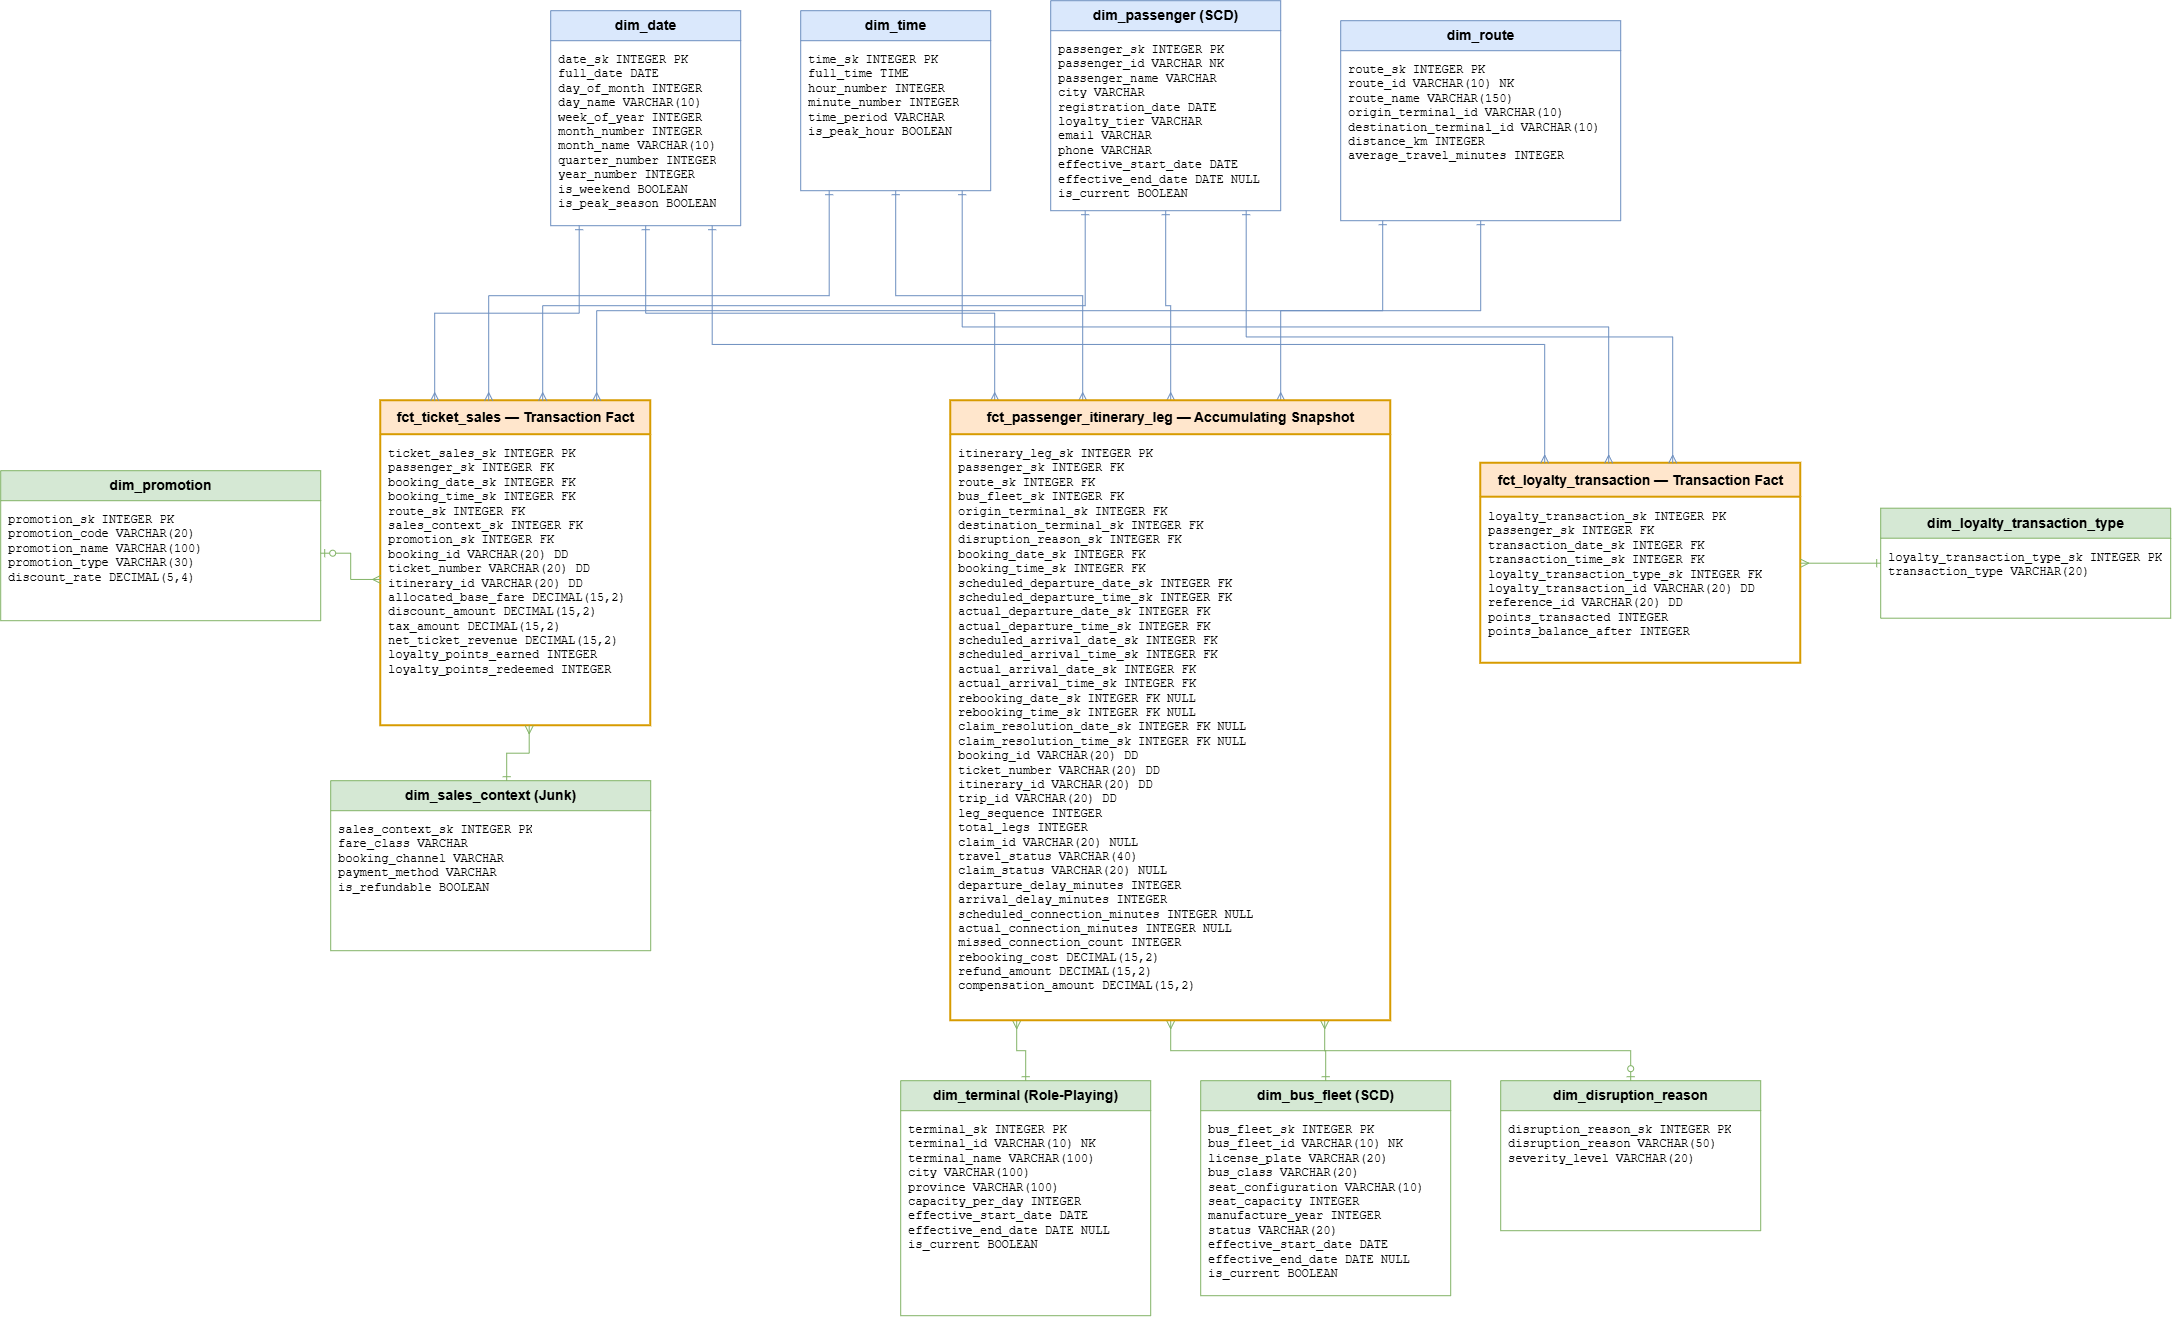
\includegraphics[width=0.97\textwidth,height=0.75\textheight,keepaspectratio]
{figures/dimension_full.drawio.png}

\footnotesize Diagram lengkap mencantumkan kolom, tipe data utama, primary key,
dan foreign key.
\end{frame}

\begin{frame}{Slowly Changing Dimension}
\footnotesize
\begin{itemize}
    \item \texttt{dim\_passenger.loyalty\_tier}: SCD Tipe 2 agar tingkat
    loyalitas pada waktu transaksi tetap dapat diketahui.
    \item \texttt{dim\_bus\_fleet.bus\_class} dan konfigurasi kursi: SCD Tipe 2
    agar kapasitas historis tidak berubah ketika armada diperbarui.
    \item Koreksi atribut kontak atau kesalahan administratif: SCD Tipe 1.
\end{itemize}

\begin{block}{Kontrol versi SCD Tipe 2}
Natural key, surrogate key, tanggal mulai, tanggal akhir, dan penanda versi aktif.
\end{block}
\end{frame}

\section{Data Sintetis dan ETL}

\begin{frame}{Pembuatan Data Sintetis}
\footnotesize
\begin{columns}[T]
\column{0.58\textwidth}
\begin{itemize}
    \item Generator dibuat dengan Python, pandas, NumPy, dan Faker.
    \item Seed tetap digunakan agar hasil dapat diulang.
    \item Terdapat musim sibuk, perjalanan multi-leg, keterlambatan ekstrem,
    data kontak kosong, klaim, dan perubahan atribut SCD.
    \item Data mentah disimpan sebagai CSV dan tidak diubah oleh ETL.
\end{itemize}
\column{0.37\textwidth}
\begin{block}{Volume utama}
\centering
15 tabel sumber\\[0.2cm]
25.000 tiket-leg\\[0.2cm]
lebih dari 10.000 transaksi
\end{block}
\end{columns}
\end{frame}

\begin{frame}{Alur ETL}
\footnotesize
\centering
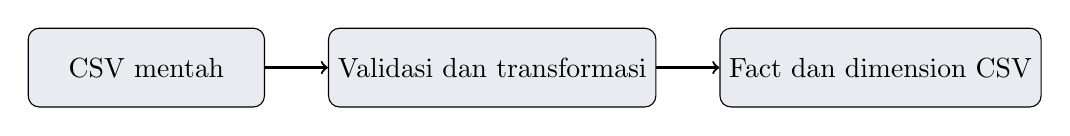
\begin{tikzpicture}[node distance=0.8cm]
\node[draw,rounded corners,fill=ugmblue!10,minimum width=3cm,
minimum height=1cm] (raw) {CSV mentah};
\node[draw,rounded corners,fill=ugmblue!10,right=of raw,minimum width=4cm,
minimum height=1cm] (transform) {Validasi dan transformasi};
\node[draw,rounded corners,fill=ugmblue!10,right=of transform,minimum width=4cm,
minimum height=1cm] (mart) {Fact dan dimension CSV};
\draw[->,thick] (raw) -- (transform);
\draw[->,thick] (transform) -- (mart);
\end{tikzpicture}

\vspace{0.6cm}
\begin{itemize}
    \item Surrogate key dibentuk dan lookup SCD dilakukan sesuai tanggal transaksi.
    \item Foreign key dan grain diperiksa sebelum data ditulis.
    \item Baris yang melanggar kapasitas perjalanan dipindahkan ke keluaran
    \textit{rejected}, bukan dihapus dari data mentah.
\end{itemize}
\end{frame}

\begin{frame}{Hasil Akhir Data Mart}
\footnotesize
\begin{columns}[T]
\column{0.48\textwidth}
\begin{block}{Dimension table}
10 tabel, antara lain penumpang, tanggal, waktu, terminal, rute, dan armada.
\end{block}
\begin{block}{Dokumentasi}
\texttt{schema.sql} dan data dictionary untuk seluruh tabel dan kolom.
\end{block}
\column{0.48\textwidth}
\begin{block}{Fact table}
\begin{tabular}{lr}
Penjualan tiket & 25.000 \\
Itinerary leg & 24.980 \\
Loyalitas & 13.928 \\
\end{tabular}
\end{block}
\begin{block}{Rekonsiliasi itinerary leg}
25.000 mentah = 24.980 dimuat + 20 ditolak.
\end{block}
\end{columns}
\end{frame}

\section{Verifikasi}

\begin{frame}{Cara Verifikasi}
\footnotesize
\begin{enumerate}
    \item CSV data mart dimuat ke SQLite \textit{in-memory} melalui notebook.
    \item Lima query SQL dijalankan untuk menjawab lima business questions.
    \item Hasil query ditampilkan sebagai tabel.
    \item Sebelas pemeriksaan kualitas data dijalankan untuk memeriksa duplikasi,
    nilai kosong tak terduga, foreign key, grain, dan versi SCD.
\end{enumerate}

SQLite hanya digunakan untuk verifikasi; keluaran utama data mart tetap berupa CSV.
\end{frame}

\begin{frame}{Temuan Operasional}
\footnotesize
\begin{columns}[T]
\column{0.49\textwidth}
\begin{block}{Missed connection tertinggi}
Pati: Cilacap--Pati dilanjutkan Pati--Jakarta\\
273 dari 285 koneksi (95,79\%).
\end{block}
Lima pasangan teratas memiliki tingkat 84,23--95,79\%.
\column{0.47\textwidth}
\begin{block}{SLA breach tertinggi}
Jakarta--Surabaya, BUS-071 (Executive)\\
Rata-rata terlambat 115,33 menit; 66,67\% dari 3 perjalanan.
\end{block}
Jumlah perjalanan perlu diperhatikan karena beberapa kombinasi hanya memiliki
sedikit observasi.
\end{columns}
\end{frame}

\begin{frame}{Temuan Finansial dan Loyalitas}
\footnotesize
\begin{itemize}
    \item \textit{Revenue leakage} musim sibuk tertinggi ditemukan pada rute
    Salatiga--Jepara, sebesar Rp56.653.000.
    \item Tingkat Basic mencatat 8.254 pemesanan dari 2.749 penumpang, dengan
    rata-rata frekuensi 3,00 pemesanan per penumpang.
    \item Kelompok yang pernah mengalami \textit{missed connection} memiliki
    \textit{repeat booking rate} 94,85\%, dibandingkan 76,54\% pada kelompok tanpa
    gangguan.
\end{itemize}

\begin{alertblock}{Interpretasi}
Hasil terakhir tidak membuktikan bahwa gangguan meningkatkan loyalitas. Penumpang
yang lebih sering bepergian memiliki peluang lebih besar untuk mengalami gangguan
sekaligus melakukan pemesanan berulang.
\end{alertblock}
\end{frame}

\begin{frame}{Data Quality Check}
\footnotesize
\begin{columns}[T]
\column{0.53\textwidth}
Pemeriksaan mencakup:
\begin{itemize}
    \item duplikasi primary key dan grain;
    \item foreign key tanpa pasangan;
    \item nilai wajib yang kosong;
    \item rentang versi SCD yang tumpang tindih; dan
    \item rekonsiliasi baris mentah, dimuat, dan ditolak.
\end{itemize}
\column{0.42\textwidth}
\begin{block}{Hasil}
\centering
11 pemeriksaan\\[0.3cm]
seluruhnya menghasilkan\\[0.2cm]
\Large\textbf{0 masalah}
\end{block}
\end{columns}
\end{frame}

\section{Visualisasi Tableau}

\begin{frame}{Kinerja Operasional dan Dampak Finansial}
\centering
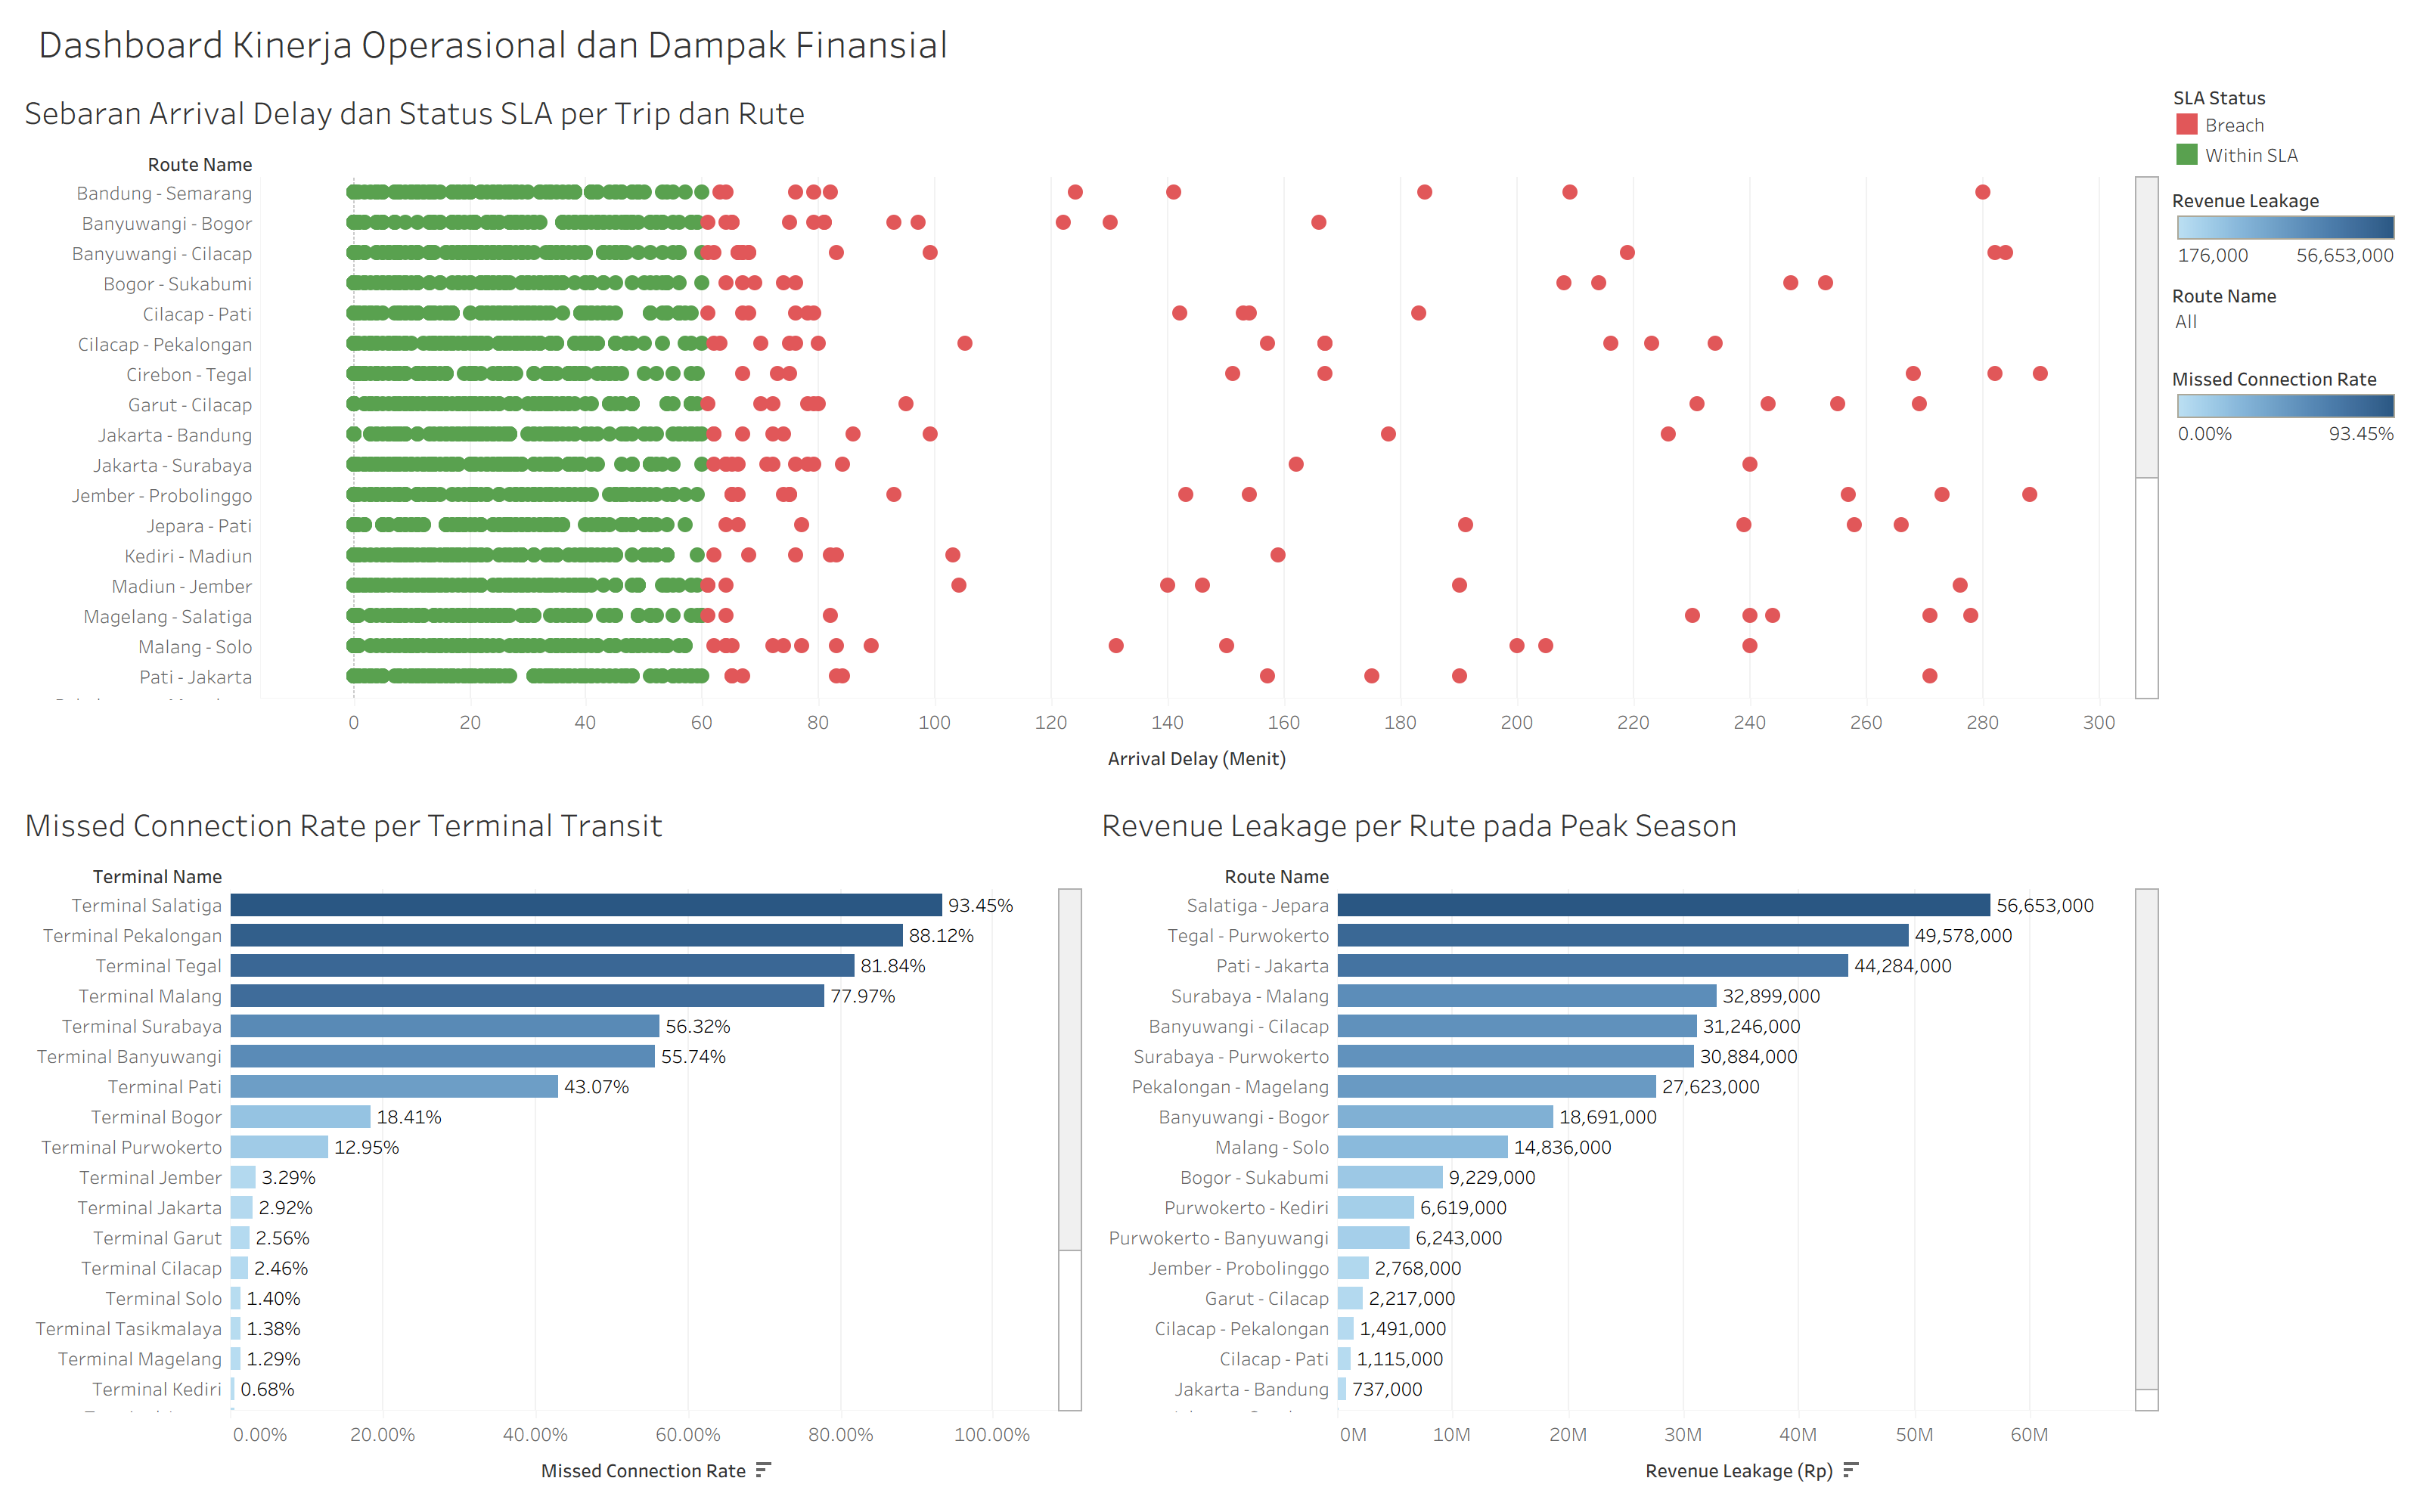
\includegraphics[width=0.96\textwidth,height=0.72\textheight,keepaspectratio]
{figures/dashboard-operasional.png}

\scriptsize Terminal Salatiga memiliki \textit{missed connection rate} tertinggi
(93,45\%), sedangkan \textit{revenue leakage} terbesar terdapat pada rute
Salatiga--Jepara (Rp56.653.000).
\end{frame}

\begin{frame}{Loyalitas dan Perilaku Penumpang}
\centering
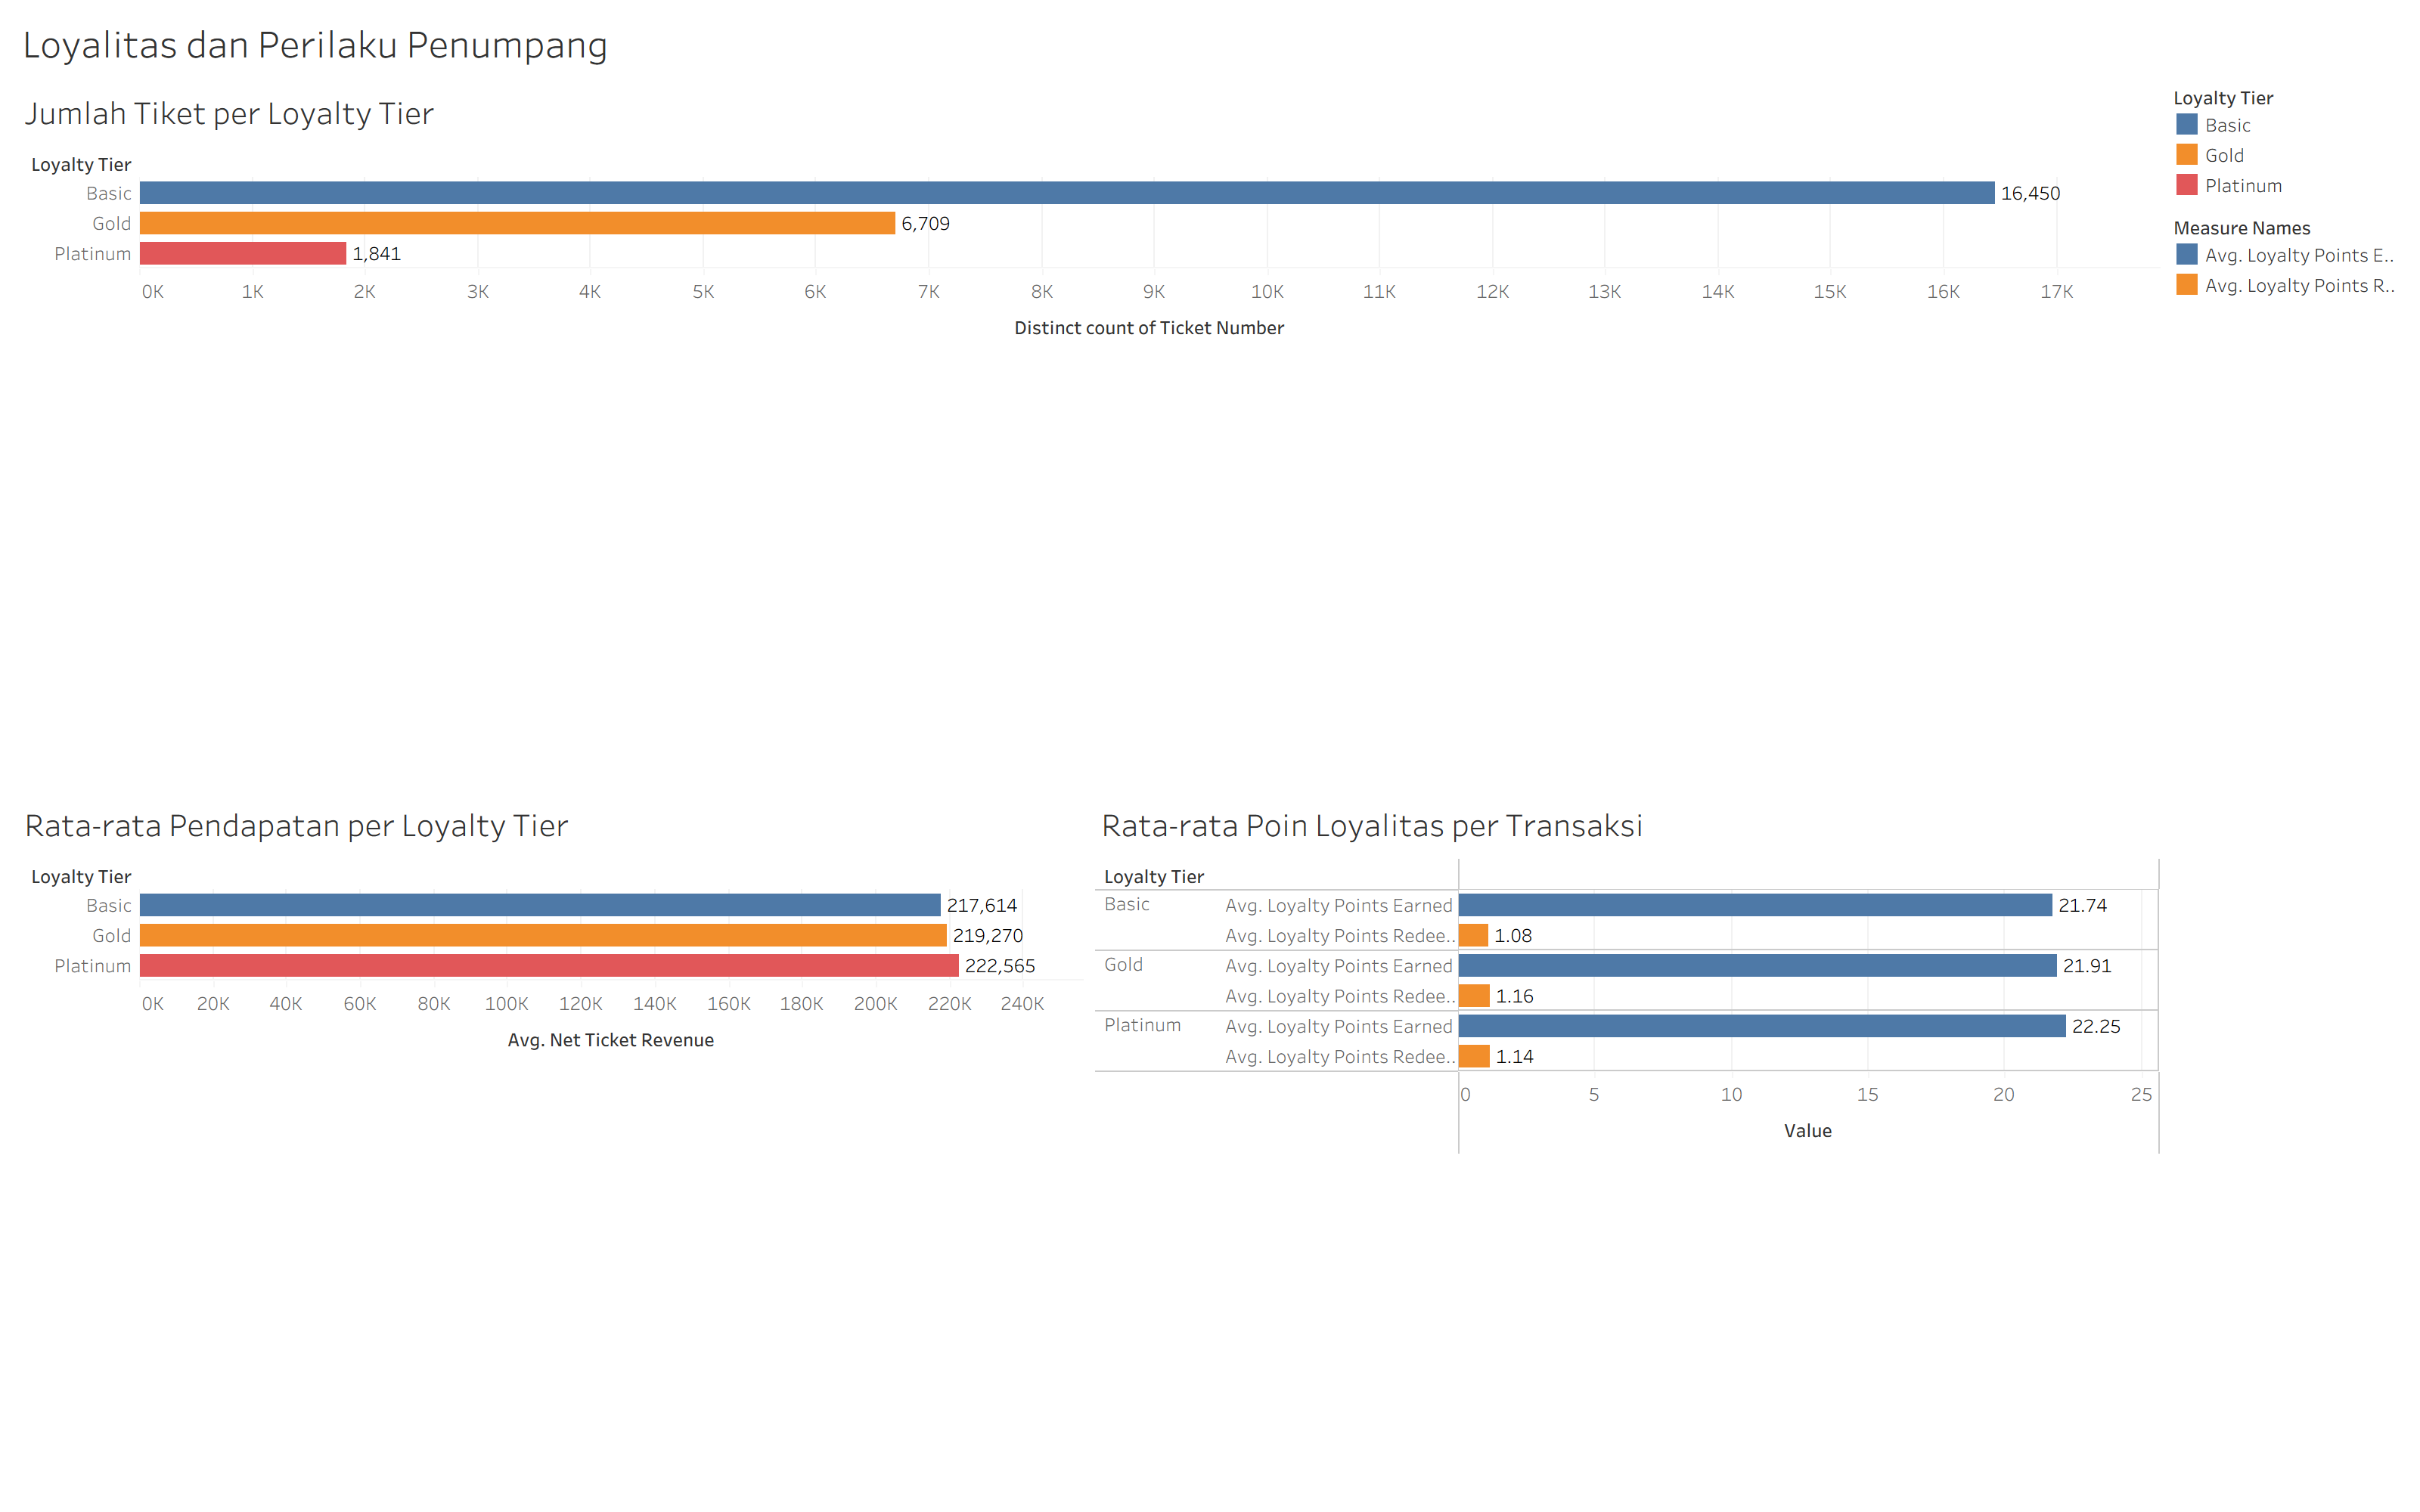
\includegraphics[width=0.96\textwidth,height=0.72\textheight,keepaspectratio]
{figures/dashboard-perilaku-loyalitas.png}

\scriptsize Tier Basic mencatat jumlah tiket terbesar, sedangkan Platinum memiliki
rata-rata pendapatan tiket tertinggi sebesar Rp222.565.
\end{frame}

\begin{frame}{Aktivitas Transaksi Loyalitas}
\centering
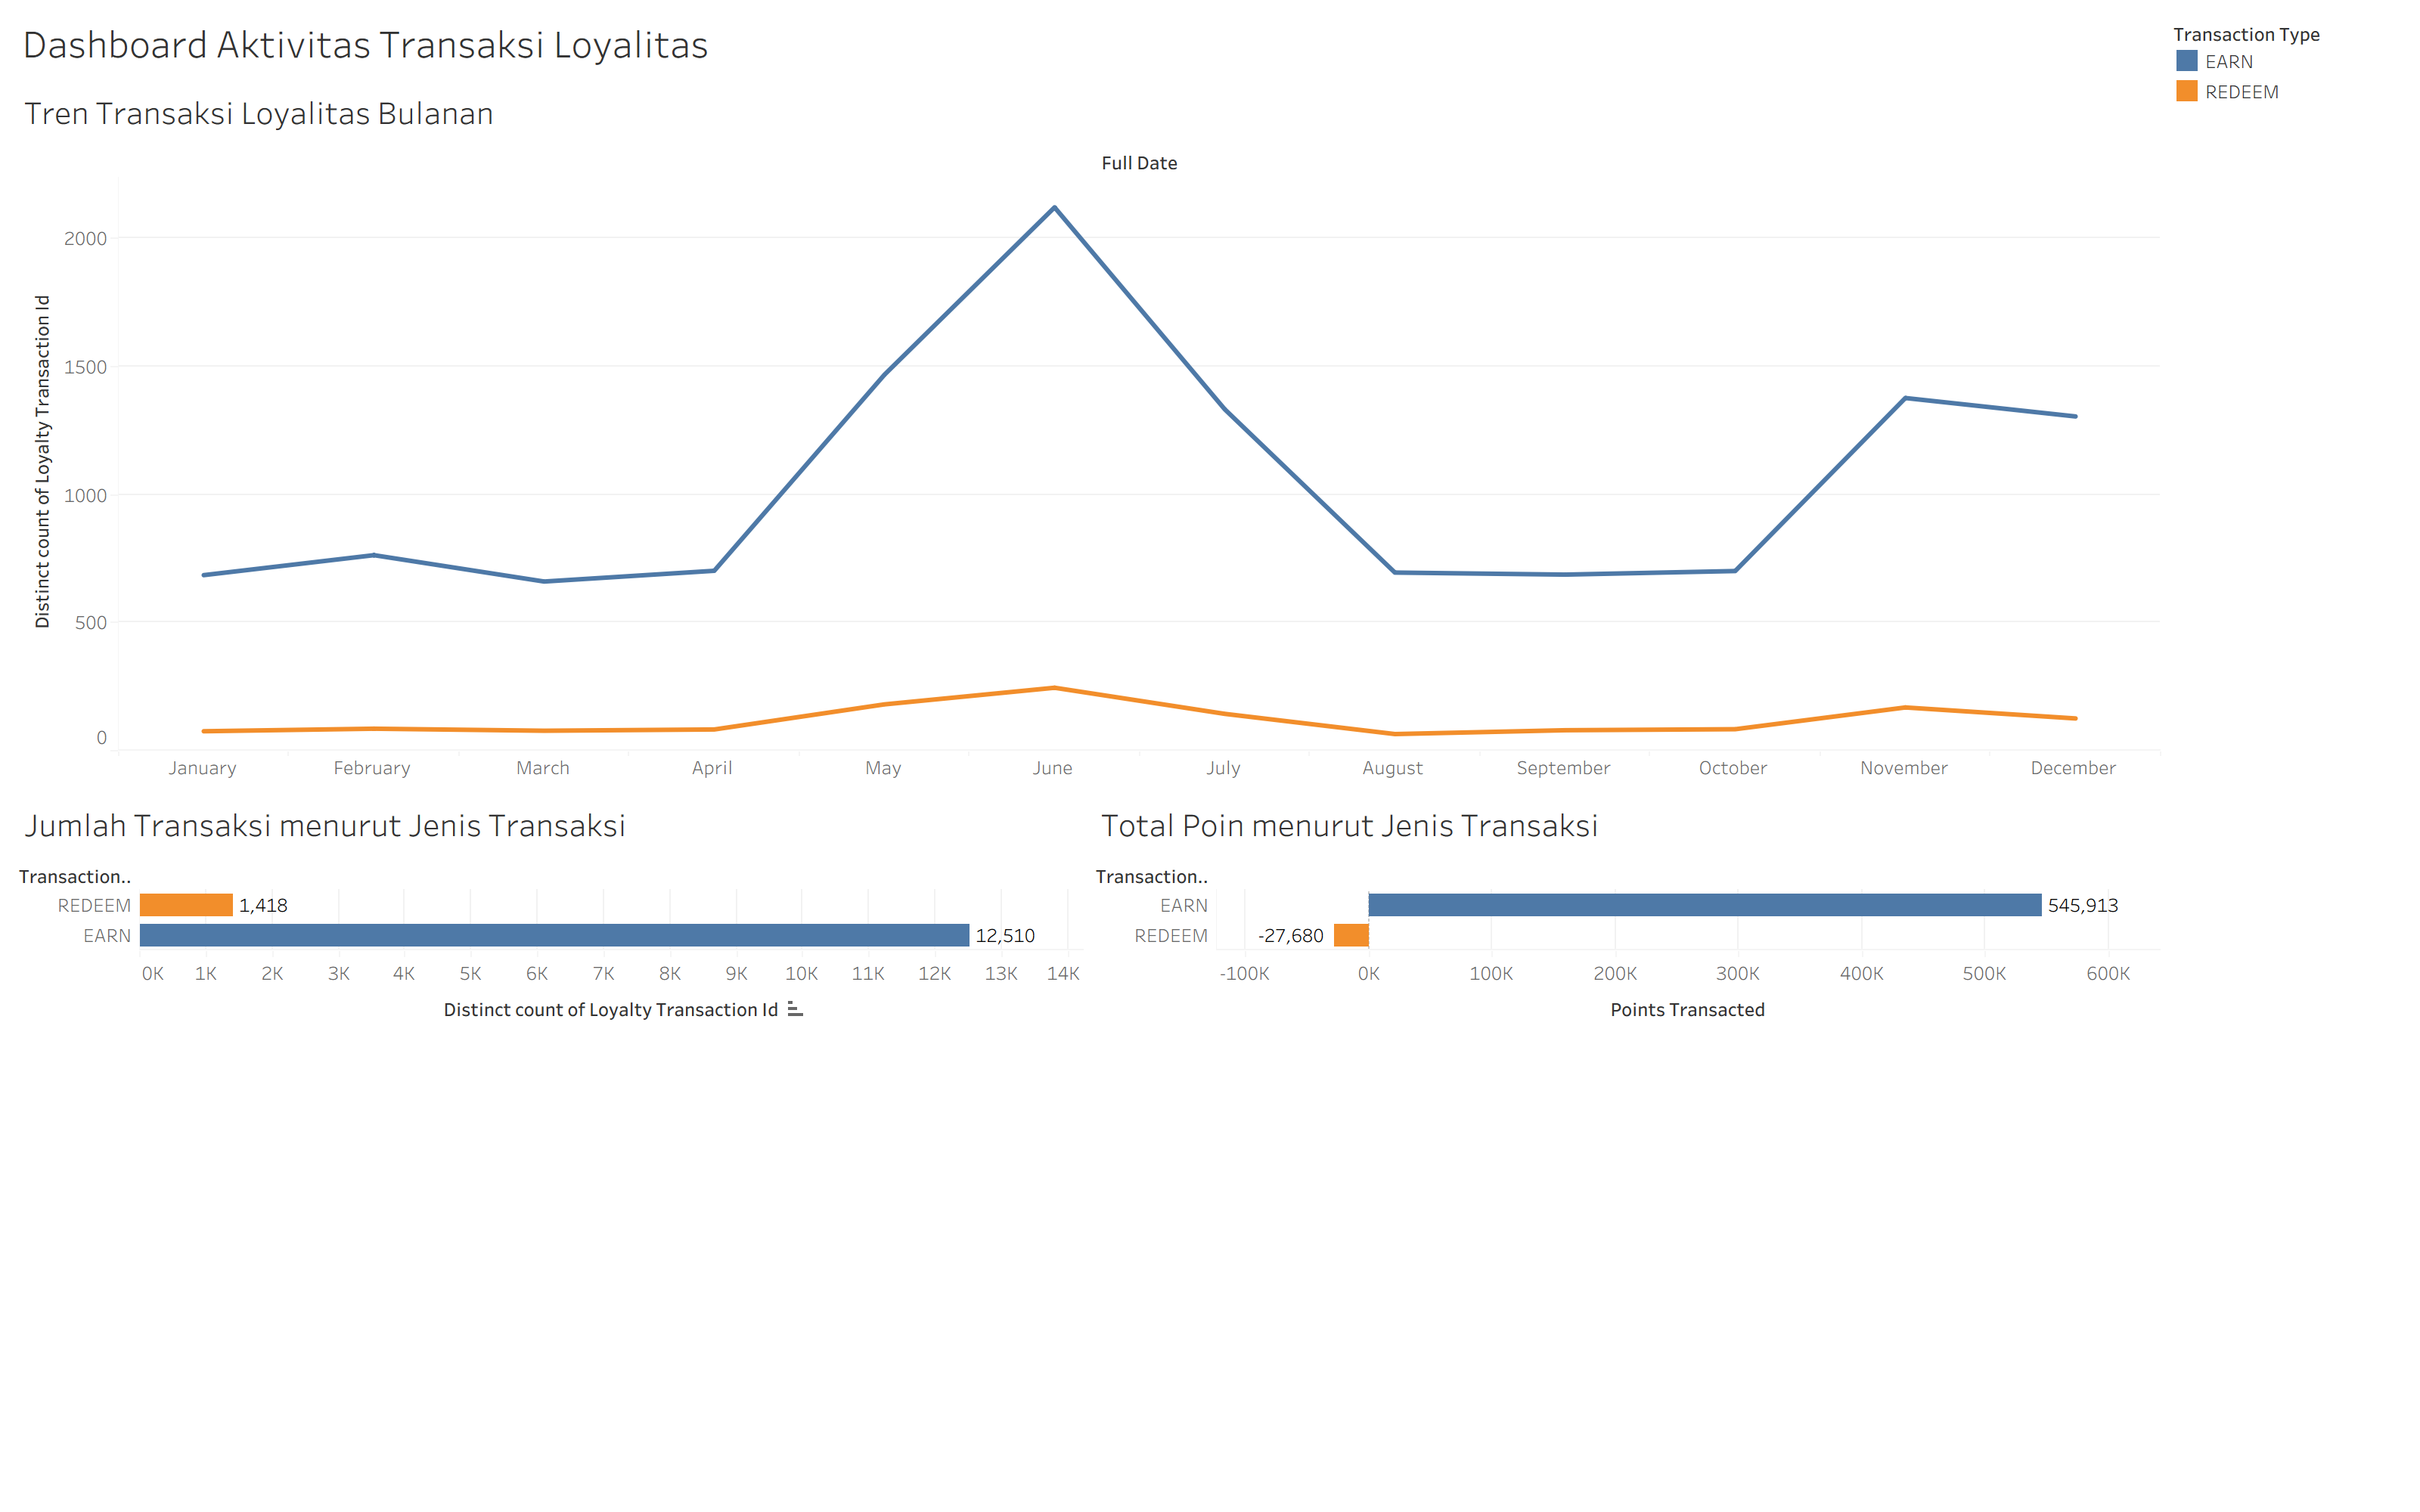
\includegraphics[width=0.96\textwidth,height=0.72\textheight,keepaspectratio]
{figures/dashboard-transaksi-loyalitas.png}

\scriptsize Terdapat 12.510 transaksi \texttt{EARN} dan 1.418 transaksi
\texttt{REDEEM}. Aktivitas meningkat pada Juni serta November--Desember.
\end{frame}

\section{Penutup}

\begin{frame}{Kesimpulan}
\footnotesize
\begin{itemize}
    \item Tiga proses bisnis dipisahkan ke dalam tiga fact table dengan grain yang
    jelas dan conformed dimensions.
    \item Generator menghasilkan variasi untuk menguji SCD, gangguan perjalanan,
    dan masalah kualitas data.
    \item ETL menghasilkan data mart CSV yang terdokumentasi dan lolos pemeriksaan
    integritas referensial.
    \item Lima query menjawab pertanyaan bisnis, tetapi hasil asosiasi perlu
    ditafsirkan dengan memperhatikan frekuensi perjalanan.
    \item Tiga dashboard Tableau menunjukkan bahwa seluruh fact table dapat
    digunakan untuk analisis operasional, komersial, dan loyalitas.
\end{itemize}
\end{frame}

\begin{frame}[c]{Diskusi}
\centering
\Huge\color{ugmblue}\textbf{Terima Kasih}
\end{frame}
\end{document}
